
Machine Learning (ML) can be defined as an application of Artificial Intelligence that permits the computer system to learn without being told explicitly. 
In ML a computer program is said to learn from experience E with respect to some class of tasks T and performance measure P, if its performance at tasks in T, as measured by P, improves with experience E \cite{Coursera}.
 ML has made tremendous strides in the past decades and has become very popular recently due to its multifaceted applications. It is being used on social media, marketing, and in the scientific community as well. 
Some examples of ML applications are: the algorithms used on application in smartphones to detect human faces, self-driving cars, computer games, stock prediction, and voice recognition. An interesting characteristic of ML algorithms is that the more data one inputs the better is the performance. The ML application has a very wide spectrum covering almost every aspect of human endeavor that involves a lot of data. 
Scientific analysis today generates enormous data and is a hence is a perfect used case to apply ML techniques. In this work we use enhanced ML techniques based on progress in the recent past.

In general, there are two main categories to classify machine learning problems: \textbf{Supervised Learning} (SL) and \textbf{Unsupervised Learning} (UL). SL is the most used ML approach and has proven to be very effective for a wide variety of problems. Examples of common SL problems are: spam filters, predicting housing prices, identifying a malignant or benign tumor, etc. These types of problems are characterized by providing a “right answer” as a reference. For example, spam filter algorithms identify emails that are spams by training on a dataset that has examples of such emails. In case of predicting house prices, the algorithm is trained on a dataset of houses involving features like the area of the house, number of rooms, and the selling price of the house.

UL algorithms are different in the sense that they do not have the “right answers” given to the machine. Instead, UL algorithms are used for finding patterns and make clusters from the given data. That is what also forms the basis of a search engine (e.g. Google news). Clicking on a link to a news article, one gets many different stories of different journals that have some correlation with the article searched. This happens because the ML algorithm is capable of learning features and shared patterns from a bunch of data without being given any specifics. Another interesting UL problem is the so-called “cocktail party” that involves distinguishing the voice of two people recording on two microphones located at different places. The ML algorithm is able to separate the sources of the voices in the recordings by learning the voice features that correspond to each person, showing the power of the UL algorithm.

In this study, I have focused on an SL approach and a variant of the UL approach, called the \textbf{Semi-Supervised Learning} approach (SSL). The SSL is named so because the data involves looking at images that are already known to be “Good” but one doesn’t necessarily know every possible situation that produces a “Bad” image. The purpose is to define a metric for a “good” image and subsequently decide if an image is “bad” in case it deviates too much from an acceptable value.



\section{Developing the Algorithm}

To develop an ML algorithm the following are taken into consideration, what is the task? and what is the method to approach the task? In our case, we are looking into images that have information about the activity that the channels in the HCAL are detecting. These images are called "occupancy maps" and they are a visual way of monitoring the health of the detector itself (see \autoref{Occupancymaps5x5}). There are two common problems that can be identified by viewing occupancy maps which are called "dead channels" and "hot towers". They are referred to as “dead” and “hot” respectively in the rest of this document. Dead channels mean that on a certain place in the occupancy map there is not any readout from the channels on the HCAL and hot channels mean that there are channels that are being triggered by noise or are damaged in a way that makes them readout too much activity.

\begin{figure}[h]
\begin{subfigure}{.3\textwidth}
	\centering
	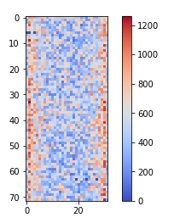
\includegraphics[width=.8\textwidth]{Good_image.jpg}
	\caption{Good Image\label{Goodimage}}
\end{subfigure}
%
\begin{subfigure}{.3\linewidth}
	\centering
	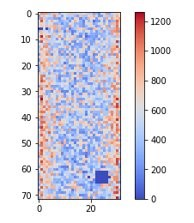
\includegraphics[width=.89\linewidth]{Dead_image_5x5.jpg}
	\caption{Dead Image \label{Deadimage}}
\end{subfigure}
%
\begin{subfigure}{0.3\linewidth}
	\centering
	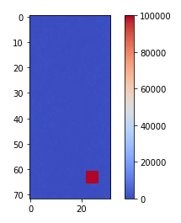
\includegraphics[width=.84\linewidth]{Hot_image_5x5.jpg}
	\caption{Hot Image \label{Hotimage}}
\end{subfigure}
\vspace{1cm}
\caption{Occupancy maps with 5x5 affected regions \label{Occupancymaps5x5}}
\end{figure}

The problem is the following, to create a model that can detect and classify what type of scenario is occurring on each occupancy map. For this, we want to go with a SL approach which means that we will give the model the images as the input and it will train on these images by learning to identify patterns or features in the image and try to do a “fit” from the images to their corresponding labels. After the training, the algorithm will be given a testing set for us to evaluate the model’s ability to correctly detect if there is a problem with the image and what type of problem is being detected. The output of the model will be the predicted class of the test image. The predictions are based on the labels and their corresponding images that were given to the model during training. This means that if the model was trained with 3 different types of images with their corresponding label the model will only work well for images that present similar patterns or characteristics to those presented in the training. For example, if we only train the model to distinguish between “good” and “hot” then when the model encounters images that aren’t either of these two, like an image labeled “dead”, then the model will not know what to do with this image and will give it an incorrect label.
After the SL model has been tested the next step is trying an SSL model. The term semi-supervised simply means that there isn’t a ground truth label that is being given to the model during training because either there isn’t necessarily a ground truth, or we don’t know what the ground truth is. What we do know, is what is considered as a “good” image and what this approach hopes to accomplish is to use the error in the reconstruction of the input image and use that information to discriminate between the “good” vs the “bad” images.

\section{Teaching the Algorithm}

The way an ML algorithm learns is by an iterative process called an optimization algorithm in which the predicted output value of the model is compared to the desired output (See \autoref{WandB}) and the weights and biases of the model are adjusted such that the predicted output is closer to the desired output.

\begin{figure}[th]
\centering
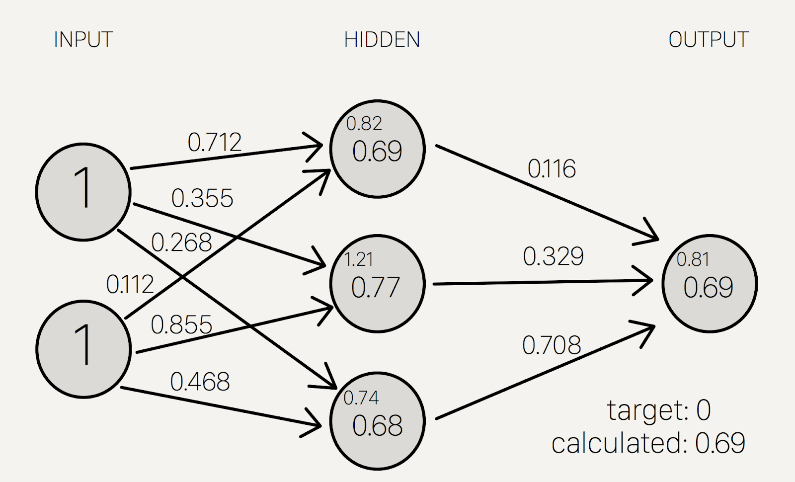
\includegraphics[width=.68\textwidth]{Weights_and_biases.png}
\caption{Weights and Biases \label{WandB}}
\end{figure}

“Optimization algorithms helps us to \textbf{minimize} (or \textbf{maximize} ) an \textbf{Objective} function \textit{(another name for \textbf{Error} function)} \textbf{E(x)} which is simply a mathematical function dependent on the Model’s internal \textbf{learnable parameters} which are used in computing the target values(\textbf{Y}) from the set of \textit{predictors}(\textbf{X}) used in the model. For example — we call the \textbf{Weights(W)} and the Bias(b) values of the neural network as its internal learnable parameters which are used in computing the output values and are learned and updated in the direction of optimal solution i.e. minimizing the Loss by the network’s training process and also play a major role in the training process of the Neural Network Model.” (Walia, 2018).
The most basic and probably the most used optimizer is called Gradient Descent (GD). GD is based on the concept of using the gradient of a loss or cost function and moving the weights and biases of the ML model so that the predicted value is taking a step in the decreasing direction of this error function (See Figure 5). In general, the “terrain” of the loss function is not a smooth bowl-shaped surface like the one present in the image. The most general form of the surface is more similar to a rocky mountain (See Figure 6), which presents a problem when using simple optimizers like GD.






